\section{Globales FEM}
Wie in der Aufgabenstellung beschrieben, soll zur Überprüfung der Handrechnungen ein gloables FEM-Modell zur Anwendung kommen. In diesem Kapitel wird nun beschrieben, wie dieses FEM-Modell aufgesetzt und welche Annahmen getroffen werden. Weiter werden die Ergebnisse der Simulationen aufgeführt, mit den Handrechnungen verglichen und beurteilt.\\

Es werden vier Berechnungen gemacht wie in den Handrechnungen. Wieso genau diese vier?

Mit dem globalen FEM-Modell sollen folgende Punkte bestimmt werden:
\begin{itemize}
  \item Lagerreaktionen
  \item Maximale Axialkräfte, Querkräfte und Biegemomente in Chassis, Dach und derTrägern A und B
  \item Kontaktreaktion: Chassis zu Träger A und B
  \item Kontaktreaktion: Chassis zu Boden
  \item Deformation
\end{itemize}

\subsection{Idealisierung und Modell}
Das FEM-Modell des Solar Butterflys wird aus Balken und Schalenkörper aufgebaut. Das Chassis, die Träger A und B sowie die Dachträger werden als Balken mit den entsprechenden Querschnitten modeliert. Die Wände, Dächer und der Boden werden das Schalenkörper modelliert, wobei den Schalenkörper jeweils ein Lagenaufbau zugewiesen wird, welcher die Sandwichbauweise nachstellt. In den Abbildungen \ref{FEM Mesh1} ist das komplette Modell des Solar Butterflys zu sehen. In der Abbildung \ref{FEM Mesh3} wurden die Schalenkörper ausgeblendet, sodass nur die Balken sichtbar sind.

\begin{figure}[H]
  \centering
  \centering
  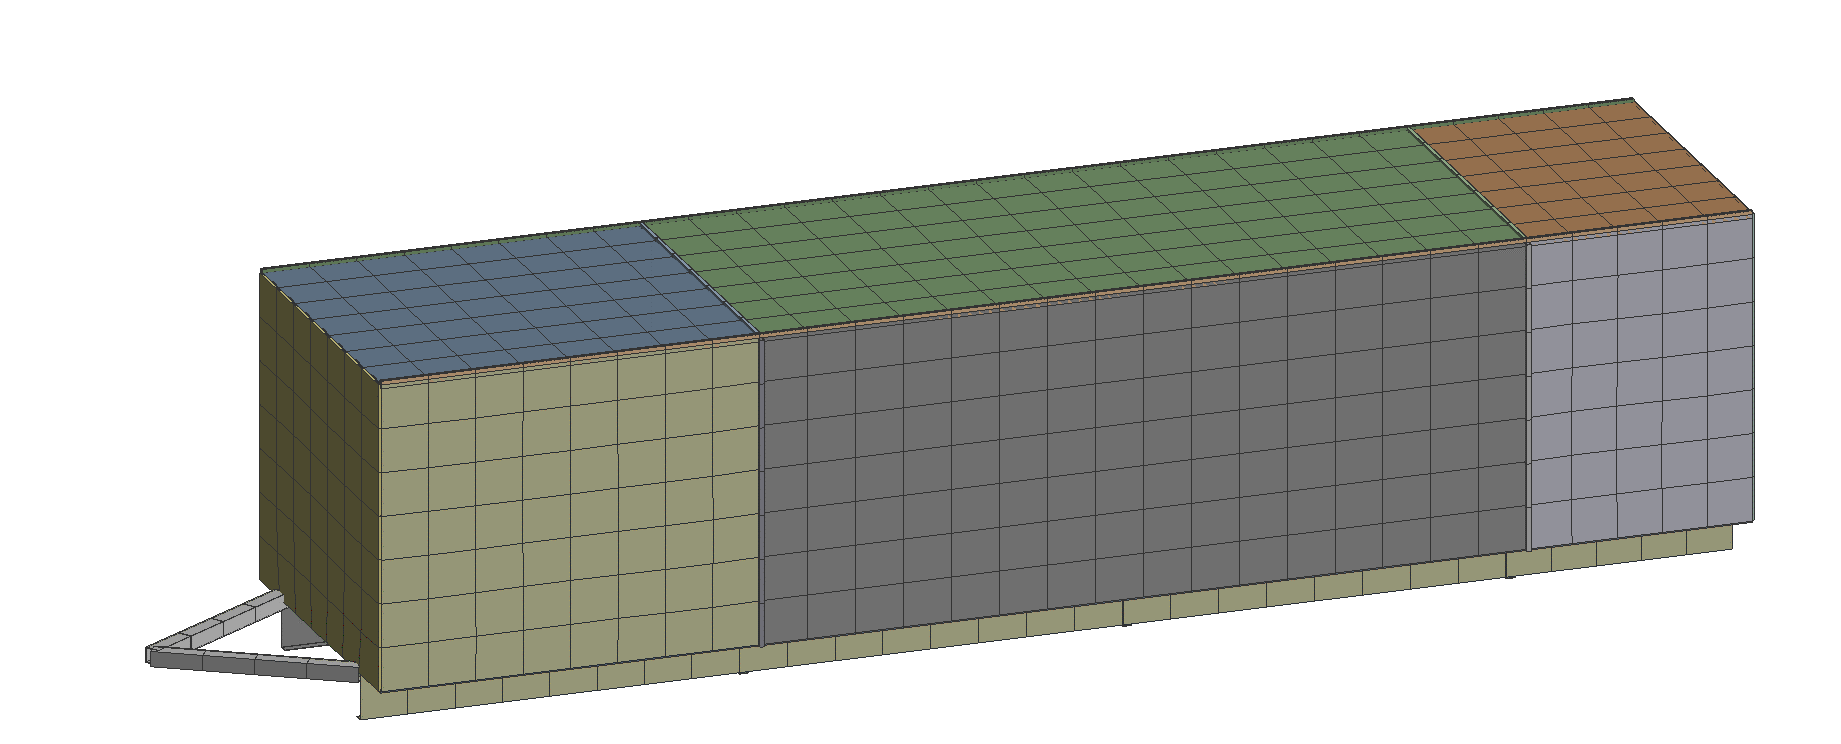
\includegraphics[width=.7\linewidth]{04_figures/FEM Mesh1.png}
  \caption{Darstellung der Balken und Schalenkörper im FEM-Modell}
  \label{FEM Mesh1}
\end{figure}
\begin{figure}[H]
  \centering
  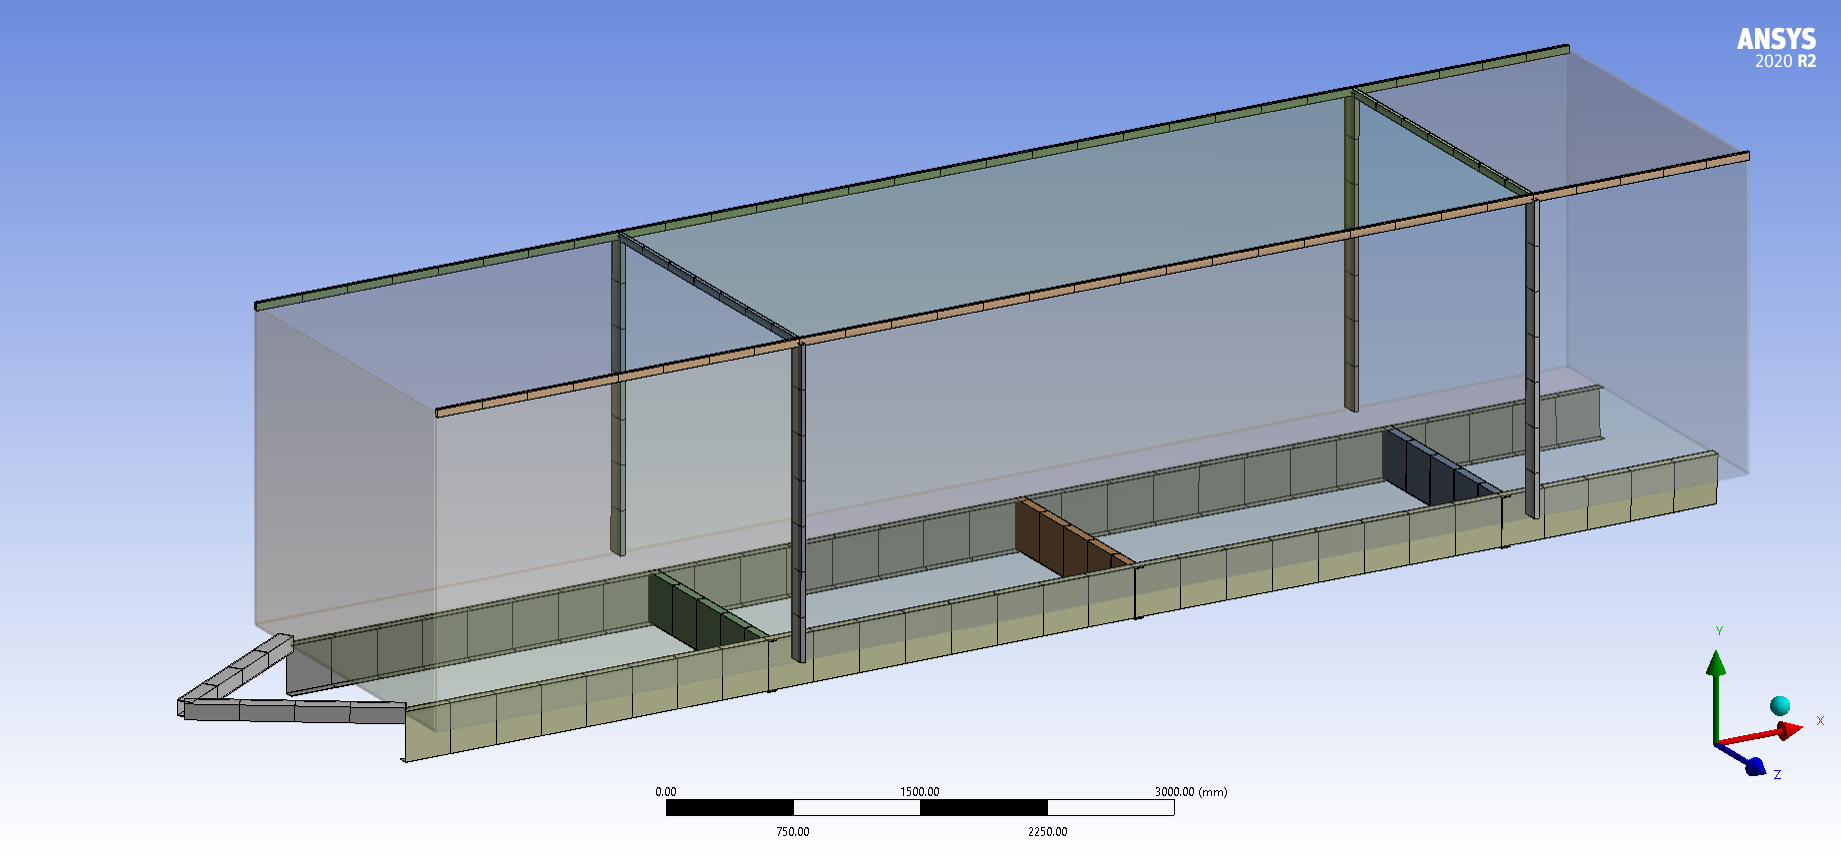
\includegraphics[width=.7\linewidth]{04_figures/FEM Mesh3.png}
  \caption{Darstellung der als Balken idealisierten Körper}
  \label{FEM Mesh3}
\end{figure}

Um die Masse des Solar Butterflys modellieren zu können, werden, zusätzlich zu den Massen der modellierten Bauteilen, Punktmassen (Point-mass) eingeführt. Es werden für die drei Raumelemente Küche, Mittelkörper und Bad je eine Punktmasse definiert, deren Masse und Trägheitsmomente mit der Hilfe der Massenverteilung aus dem Kapitel KAPITEL bestimmt werden. In der Abbildung \ref{img:FEM Punktmasse} sind die Verbindung der Punktmassen mit dem Rest des Modelles dargestellt.\\
\begin{figure}[h]
  \centering
  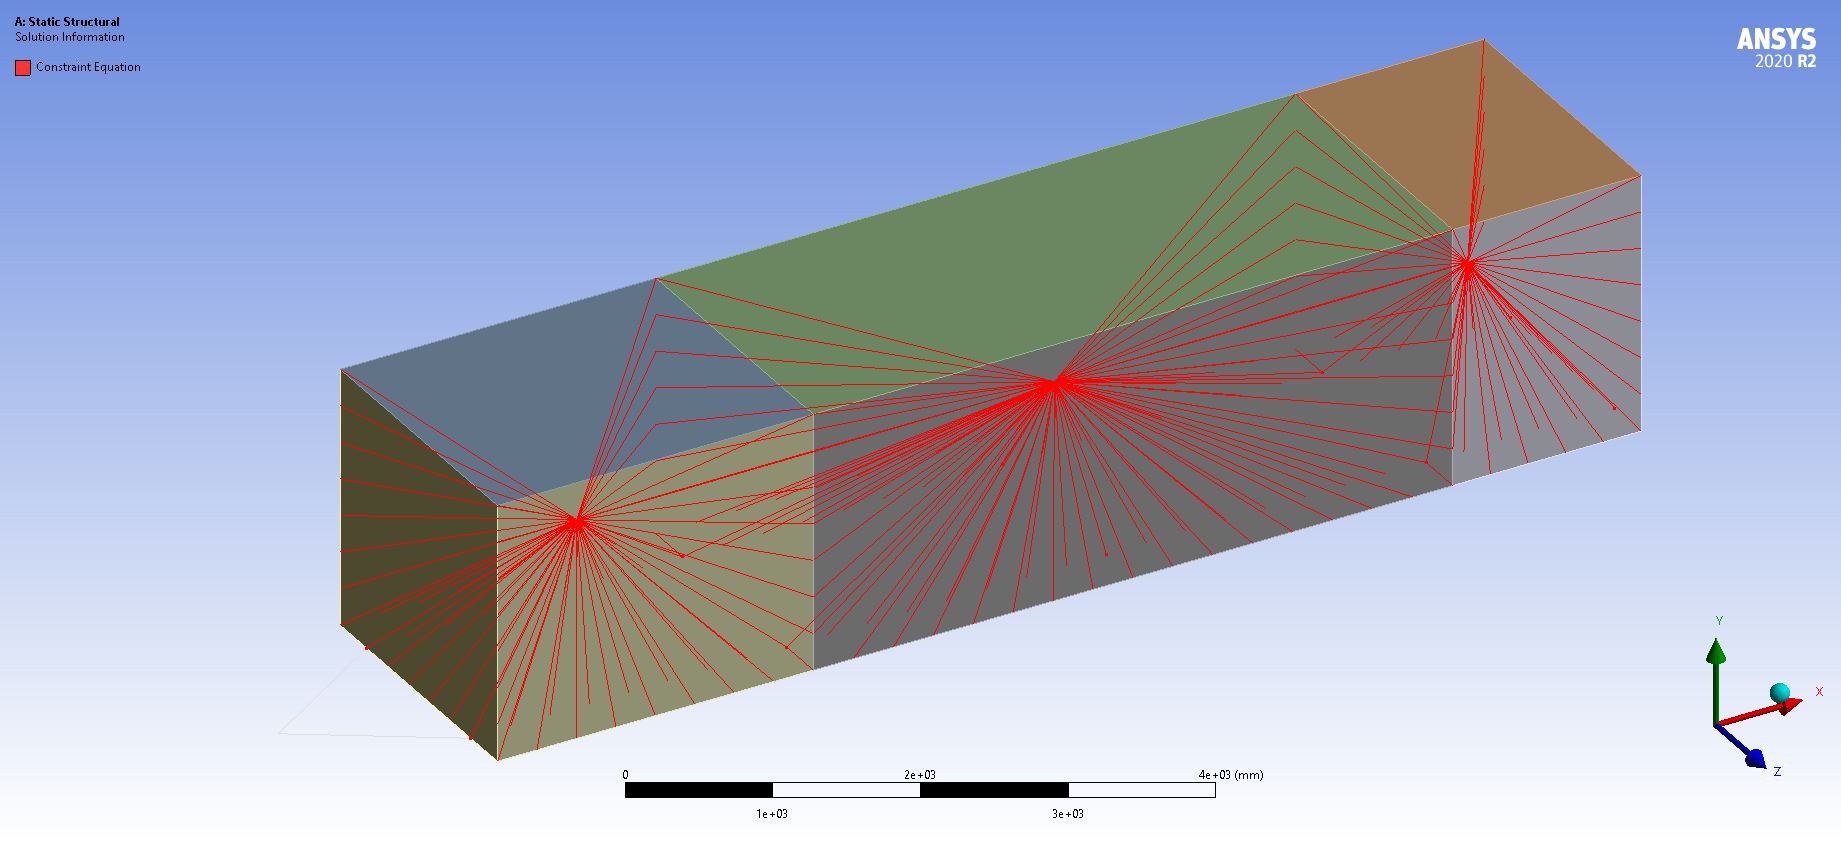
\includegraphics[width=0.7\linewidth]{04_Figures/FEM Punktmasse.png}
  \caption{Verbindungen der Punktmassen zum Rest des Modelles}
  \label{img:FEM Punktmasse}
\end{figure}

Die Deichsel, Längsträger und Querträger des Chassis werden durch das Zusammenführen der deckungsgleichen Koten miteinander verbunden. Auf die selbe Art und Weise werden die Träger A und B, die Träger des Daches sowie der Boden, die Wände und das Dach des Aufbaus miteinander verbunden. Der nun verbundene Aufbau wiederum wird auf zwei Arten mit dem Chassis verbunden. Einerseits werden die Träger A und B über Fixe MPC-Kontakte (alle Freiheitsgrade eingeschränkt) an ihrem untersten Knoten mit dem Chassis verbunden. Weiter wird der Boden über Translatorische MPC Kontakte mit den Längsträgern des Chassis verbunden. Sie räpresentieren die Klebestellen zwischen Boden und Chassis. Mit dem Auslesen der Kontaktreaktionen dieser beiden Verbindungen können Aussagen bezüglich der Verbindung zwischen den Trägern A und B und dem Chassis, sowie auch der Klebestelle zwischen dem Chassis und Boden gemacht werden.\\
In allen folgenden FEM-Simulationen ist der Solar Butterfly analog zu den Berechnungen im Kapitel \ref{sub:Longitudinale Beschleunigung} (Lastfall \emph{1.1 Vertikale Beschleunigung}) gelagert. Am Spitz der Deichsel sind die rotatorischen Freiheitsgrade freigegeben, die translatorischen jedoch eingeschränkt. An der Achse wird lediglich die Verschiebung in x-Richtung (Fahrtrichtung) zugelassen.


\subsection{Ergebnisse}
Im Anhang \ref{FEM Ergebnisse} sind die Ergebnisse der FEM-Berechnungen Tabelarisch festgehalten. Sofern für eine ausgelesene Grösse Handrechnungen durchgeführt wurden, sind diese ebenfalls in den besagten Tabellen zu finden, sodass diese direkt mit den Resultaten der FEM-Berechnungen verglichen werden können.\\
Im Anhang \ref{FEM Deformation} sind Bilder, welche die Deformation des Solar Butterflys dokumentieren, zu finden. Die FEM-Datei ist im elektronischen Anhang ANHANG angefügt.


\subsubsection{Vergleich mit Handrechnungen}
Im Lastfall \emph{1.1 Vertikale Beschleunigung} sind die berechneten Axialkräfte im Dach rund doppelt so hoch, wie jene des FEM-Modelles. Dies ist darauf zurück zu führen, dass das mittragende Dach, welches ebenfalls Axialkräfte aufnimmt, in den Handrechnungen nicht mit berücksichtigt wurde.\\
Im Lastfall \emph{1.4 Laterale Beschleunigung} sind die mit der FEM-Berechnung erhaltenen Axialkräfte im Chassis und den Längsträger des Daches gut drei mal höher als jene der Handrechnungen. Dies, da sich der Solar Butterfly unter lateraler Beschleunigung, nicht wie angenommen verbeigt, sondern verdreht. Die Art der Deformation ist ähnlich wie jene im Lastfall \emph{1.5 Rotatorische Beschleunigung} (vgl. Abbildung im Anhang \ref{FEM 1.4} und \ref{FEM 1.5}). Da diese grundlegende Annahme der Auswirkungen der Belastung (und der Deformation) falsch getroffen wurde, sind die Ergebnisse auch dem entsprechend unterschiedlich. Die erhaltenen Kräfte sind in ihrer Art vergleich bar mit jenen des Lastfalles \emph{1.5 Rotatorische Beschleunigung}, im Betrag liegen sie jedoch tiefer.\\



\subsubsection{Beurteilung Dach}
In der folgenden Tabelle sind die Schnittgrössen der Träger des Daches enthalten.

\begin{table}[H]
\centering
\begin{tabular}{lccccccc}
\thickhline
&	Einheit	&	1.1	&	1.2	&	1.4	&	1.5	&	Max	&	Min	\\	\hline
Axialkraft	&	N	&	2879	&	-1562	&	-2560	&	-3625	&	2879	&	-3625	\\
Querkraft	&	N	&	108	&	56	&	24	&	32	&	108	&	24	\\
Biegemoment	&	kNmm	&	42	&	17	&	13	&	19	&	42	&	13	\\	\thickhline
\end{tabular}
\caption{Schnittgrössen in den Trägern des Daches in den unterschiedlichen Lastfällen}
\label{tab:FEMres Dach}
\end{table}

Wie im Kapitel \ref{Dach} beschrieben, ist das dimensionierende Kriterium des Daches dessen Verformung aufgrund des Eigengewichtes. Dem entsprechend stellen die in der Tabelle \ref{tab:FEMres Dach} aufgeführten Schnittgrössen keine kritischen Lasten dar.\\



\subsubsection{Beurteilung Träger A und B}
In der Tabelle \ref{tab:FEMres Träger} sind die maximalen Schnittgrössen der Träger zusammengestellt.
\begin{table}[H]
\centering
\begin{tabular}{lccccccc}
\thickhline
&	Einheit	&	1.1	&	1.2	&	1.4	&	1.5	&	Max	&	Min	\\	\hline
Axialkraft	&	N	&	-10904	&	-1562	&	2684	&	-4119	&	2684	&	-10904	\\
Querkraft	&	N	&	1293	&	56	&	1067	&	1311	&	1311	&	56	\\
Biegemoment	&	kNmm	&	327	&	17	&	627	&	772	&	772	&	17	\\	\thickhline
\end{tabular}
\caption{Schnittgrössen der Träger in den unterschiedlichen Lastfällen}
\label{tab:FEMres Träger}
\end{table}

Auch diese Lasten sind für die Träger keine kritischen. Die maximale Axialkraft von -10.9 kN hat, bei einer Querschnittsfläche eines Trägers von rund 1180 $mm^2$, Druckspannungen von 9.2 MPa zur folge. Die Gefahr des Knickens ist ebenfalls nicht vorhanden, da das Profil auf mindestens zwei Seiten gestützt wird. Das Maximale Biegemoment von 772 kNmm führt, bei einem minimalen Widerstandsmoment von 11900 $mm^3$, zu Spannungen von in der höhe von 65 MPa.



\subsubsection{Verbindung Boden zu Chassis}

\begin{table}[H]
\centering
\begin{tabular}{lcccccc}
\thickhline
&	Einheit	&	1.1	&	1.2	&	1.4	&	1.5	&	Max	\\	\hline
Normalkraft (Zug)	&	N	&	883	&	35	&	1942	&	3118	&	3118	\\
Schubkraft (xz-Ebene)	&	N	&	9933	&	1733	&	10972	&	10761	&	10972	\\	\hline
Normalspannungen	&	MPa	&	0.06	&	0.00	&	0.13	&	0.21	&	0.21	\\
Schubspannungen	&	MPa	&	0.67	&	0.12	&	0.74	&	0.72	&	0.74	\\	\thickhline
\end{tabular}
\caption{Schnittgrössen und Spannungen der Verbindung zwischen Chassis und Boden in den unterschiedlichen Lastfällen}
\label{tab:FEMres Boden}
\end{table}



\subsubsection{Verbindung Träger A und B zu Chassis}
\begin{table}[H]
\centering
\begin{tabular}{lccccc}
\thickhline
Lastfall / Träger	&	Einheit	&	x	&	y	&	z	&	total	\\	\hline
1.1 A	&	\multirow{8}{*}{N}	&	-56	&	2084	&	325	&	2110	\\
1.1 B	&		&	98	&	667	&	80	&	679	\\
1.2 A	&		&	-56	&	2084	&	325	&	2110	\\
1.2 B	&		&	98	&	667	&	80	&	679	\\
1.4 A	&		&	237	&	-3577	&	1729	&	3979	\\
1.4 B	&		&	-733	&	-4221	&	1679	&	4602	\\
1.5 A	&		&	373	&	-5525	&	2346	&	6014	\\
1.5 B	&		&	-1309	&	-6399	&	2221	&	6899	\\	\hline
Max	&		&	373	&	2084	&	2346	&	6899	\\
Min	&		&	-1309	&	-6399	&	80	&	679	\\	\thickhline
\end{tabular}
\caption{Maximale Axialkräfte in den Trägern A und B in den unterschiedlichen Lastfällen}
\label{tab:FEMres Träger Axial}
\end{table}

\begin{table}[H]
\centering
\begin{tabular}{lccccc}
\thickhline
Lastfall / Träger	&	Einheit	&	x	&	y	&	z	&	total	\\	\hline
1.1 A	&	\multirow{8}{*}{kNmm}	&	-734	&	-19	&	2	&	734	\\
1.1 B	&		&	-236	&	34	&	-14	&	238	\\
1.2 A	&		&	-734	&	-19	&	2	&	734	\\
1.2 B	&		&	-236	&	34	&	-14	&	238	\\
1.4 A	&		&	1924	&	71	&	-102	&	1928	\\
1.4 B	&		&	2097	&	-251	&	95	&	2114	\\
1.5 A	&		&	2767	&	112	&	-164	&	2774	\\
1.5 B	&		0	2996	&	-452	&	159	&	3034	\\	\hline
Max	&		&	2996	&	112	&	159	&	3034	\\
Min	&		&	-734	&	-452	&	-164	&	238	\\	\thickhline
\end{tabular}
\caption{Maximale Biegemomente in den Trägern A und B in den unterschiedlichen Lastfällen}
\label{tab:FEMres Träger Moment}
\end{table}


\subsubsection{Deformationen}
Die FEM-Berechnungen zeigen, dass das Chassis, im Bezug auf das Übernehmen von Lasten, eine wichtigere Funktion übernimmt, als zuvor angenommen. Dies lässt sich unteranderem an den Abbildungen \ref{} und \ref{} anhand den Deformationen erkennen. Das Chassis verformt sich realtiv stark, während der Aufbau seine rechteckige Form nahezu bei behält. Besonders in den Lastfällen der lateralen und rotatorischen Beschleunigung ist zu erkennen, dass sich lediglich das Chassis stark verdreht, und nicht wie angenommen der komplette Körper. Dies zeigt, dass die Eigenschaft des Chassis bezüglich Steifigkeit, im vergleich zum Aufbau, eine entscheidende Rolle spielt. \\


Es ist jedoch nicht klar, ob dieses Ergebniss zum Teil auch auf die Art der Einbindung der Punktmassen zurück zu führen ist. Oder anders ausgedrückt: es ist nicht klar, ob das selbe Ergebnis erzielt werden könnte, wenn die Massen realitätsgetreuer modliert worden wären. So befindet sich ein grösserer Teil der Masse, in Form der ausfahrbaren Solarmodulen, an den Wänden des Solar Butterflys. Diese Masse muss über die Wände und Träger A und B, zu einem gewissen Ausmass auch über das Dach, getragen und auf das Chassis übertragen werden. Die Punktmassen sind jedoch fast ausschliesslich über das Chassis und die Träger A und B im Raum befestigt worden. Es ist wahrscheinlich, dass sich der Aufbau in der Realität mehr verformen würde, als dies durch die FEM-Berechnungen gezeigt wird und dass die tragende Funktion des Aufbaus dennoch nicht zu unterschätzen ist. \\
Auch wenn mit einer exakteren Modellierung gezeigt werden könnte, dass der Aufbau eine wichtigere Rolle übernimmt als dies durch die vorliegenden FEM-Ergebnissen gezeigt wird, steht fest, dass die Eigenschaften des Chassis das Ergebnis dominieren.



Die Tabelle \ref{tab:FEM 1.1} stellt eine Zusammenstellung der Resultate zur FEM-Simulation des Lastfalles \emph{1.1 Vertikale Beschleunigung} dar. Die Schnittkräfte und Kontaktreaktionen beziehen sich jeweils auf einen einzelnen Balken oder Verbindungsstelle. Die Kontaktreaktion zwischen Chassis und Boden bezieht sich auf eine einzelne Knotenverbindung. Insgesammt ist der Boden an jedem Längsträger an 30 Stellen verbunden. Über die Gurtenfläche pro Abschnitt des Chassis kann auf die Spannungen in der Verbindung geschlossen werden.\\
Bei einer Fläche von 17880 $mm^2$ pro Abschnitt ergibt sich eine maximale Normalspannung von 0.04 MPa und eine maximale Schubspannung von 0.54 MPa. Beide Werte liegen deutlich unterhalb des Design-Allowable. Hierbei muss jedoch angemerkt werden, dass lokal die Spannungen deutlich höher liegen könnten und, dass das verwendete Modell nicht geeignet ist um diese Spannungskonzentrationen zu erkennen.

\begin{table}[H]
\centering
\begin{tabular}{lccccccc}
\thickhline
Chassis	&	Einheit	&	1.1	&	1.2	&	1.4	&	1.5	&	Max	&	Min	\\	\hline
Axialkraft	&	N	&	-50730	&	6080	&	-31674	&	-44164	&	6080	&	-50730	\\
Querkraft	&	N	&	17003	&	1319	&	7163	&	10927	&	17003	&	1319	\\
Biegemoment	&	kNmm	&	16980	&	2601	&	6658	&	10218	&	16980	&	2601	\\	\thickhline
\end{tabular}
\caption{Schnittgrössen des Chassis}
\label{tab:FEMres Chassis}
\end{table}





\newpage
